% =============================================================================
%  Lagrangian formulation of a hybrid De Broglie-Bohm / stochastic
%  electrodynamics model: dynamical relaxation to the Born rule via
%  zero-point field coupling.
%
%  S. Bergamin, E. Bringa
%
%  Documento unificado (Camino A: Teorema 1 condicional, hipótesis (iv)
%  de balance detallado explícita, test diagnóstico en autoestado
%  estacionario, discusión del alcance).
% =============================================================================
\documentclass[11pt,a4paper]{article}

% --- Codificación e idioma ---------------------------------------------------
\usepackage[utf8]{inputenc}
\usepackage[T1]{fontenc}

% --- Matemática --------------------------------------------------------------
\usepackage{amsmath,amssymb,amsthm}
\usepackage{bm}

% --- Tablas y figuras --------------------------------------------------------
\usepackage{booktabs}
\usepackage{graphicx}
\usepackage{siunitx}
\sisetup{output-decimal-marker={,}}

% --- Símbolos de check/cross para tabla síntesis -----------------------------
\usepackage{pifont}
\newcommand{\cmark}{\textcolor{black}{\ding{51}}}
\newcommand{\xmark}{\textcolor{black}{\ding{55}}}
\usepackage{xcolor}

% --- Entornos teorema --------------------------------------------------------
\newtheorem{theorem}{Teorema}
\newtheorem{corollary}{Corolario}

% --- Tipografía y espaciado --------------------------------------------------
\usepackage[a4paper,margin=2.5cm]{geometry}
\usepackage{hyperref}
\hypersetup{colorlinks=true,linkcolor=blue!50!black,citecolor=blue!50!black,urlcolor=blue!50!black}

\title{Lagrangian formulation of a hybrid De Broglie--Bohm /
stochastic electrodynamics model: dynamical relaxation to the Born rule
via zero-point field coupling}
\author{S. Bergamin \and E. Bringa}
\date{Mayo 2026}

\begin{document}
\maketitle

% =============================================================================
% RESUMEN
% =============================================================================
\begin{abstract}
Se presenta un modelo híbrido que combina la mecánica de De Broglie--Bohm
con un campo estocástico de punto cero inspirado en la electrodinámica
estocástica (EDE). El objetivo es investigar bajo qué condiciones la regla
de Born puede interpretarse como un estado dinámico de equilibrio
emergente bajo la acción de un campo de vacío real. Se desarrolla el
Lagrangiano completo del sistema acoplado, se derivan las ecuaciones de
movimiento mediante el procedimiento de Euler--Lagrange, y se demuestra
que el modelo preserva la conservación de energía y la ecuación de
continuidad cuántica a orden $\lambda$. Se deriva una ley de relajación
exponencial $d\langle\bar{H}\rangle_\xi/dt\leq -\Gamma(\lambda)
\langle\bar{H}\rangle_\xi$ con $\Gamma(\lambda)=\lambda^2 D\pi^2/L^2$,
extendiendo el teorema-$H$ de Valentini al modelo híbrido, bajo cuatro
hipótesis explícitas, entre las cuales identificamos por primera vez la
condición de \emph{balance detallado del ZPF respecto de $|\psi|^2$} como
hipótesis crítica que no se sigue automáticamente del acoplamiento mínimo.

Se reportan simulaciones numéricas de alta estadística ($N_p=1000$
partículas, $N_r=20$ realizaciones independientes del ZPF) en dos
geometrías: la doble rendija (sistema abierto) y la caja cerrada
$[0,\pi]^2$ con superposición multimodal de autoestados (geometría de
Valentini--Westman). En la doble rendija, donde la condición de balance
detallado se aproxima sobre la marginal $\bar{H}_x$, la ley
$\Gamma(\lambda)\propto\lambda^2$ se verifica con $R^2=0{,}99$ y
$C=3{,}68\pm 0{,}37$. En la caja cerrada, donde la condición falla, el
acoplamiento ZPF prolonga la relajación con significancia $>5\sigma$ a
partir de $\lambda\approx 0{,}10$. Un test diagnóstico en el autoestado
estacionario $\varphi_{11}$ confirma que el campo de modos planos con
espectro de Boyer no preserva $|\psi|^2$ como estado estacionario, y que
la incorporación de una deriva osmótica de Nelson restituye parcialmente
el comportamiento esperado. Este hallazgo identifica un requisito físico
no trivial para que el programa SED reproduzca la regla de Born: la
incorporación de un mecanismo de fluctuación-disipación
---plausiblemente la radiación de reacción de Abraham--Lorentz--- que
provea la deriva osmótica faltante.

La extensión a dos partículas entrelazadas demuestra adicionalmente que
las correlaciones cuánticas no locales se preservan bajo el acoplamiento
ZPF: la anticorrelación posicional se mantiene perfecta ($E=-1$) para
paquetes bien separados incluso a $\lambda=0{,}5$, y los estados
entrelazados en caja muestran oscilaciones coherentes independientes del
acoplamiento, superando la limitación principal de la EDE pura.
\end{abstract}

% =============================================================================
% SECCIÓN 1 — INTRODUCCIÓN (reescrita Camino A)
% =============================================================================
\section{Introducción}
\label{sec:introduccion}

La interpretación de De Broglie--Bohm de la mecánica cuántica proporciona
una ontología determinista: las partículas tienen posiciones bien
definidas $q(t)$ guiadas por una función de onda real $\psi$. En este
marco, la regla de Born ---$\rho=|\psi|^2$ para el ensamble de
posiciones--- se introduce como una hipótesis estadística sobre el
ensamble inicial, en lugar de ser una consecuencia del formalismo.
Valentini~\cite{Valentini1991a,Valentini1991b} y posteriormente Valentini
y Westman~\cite{ValentiniWestman2005} demostraron que, bajo
coarse-graining, la dinámica bohmiana relaja a un equilibrio
$\bar{\rho}=|\overline{\psi}|^2$ por mezcla determinista del campo de
velocidades, dejando abierta la cuestión de si existe un mecanismo físico
subyacente que produzca relajación también a nivel fino.

La electrodinámica estocástica (EDE) propone, de manera independiente,
que los fenómenos cuánticos emergen de la interacción de partículas
clásicas con el campo electromagnético de punto cero (ZPF, del inglés
\emph{zero-point field}): un fondo de radiación Lorentz-invariante del
vacío con densidad espectral
\begin{equation}
\rho(\omega) = \frac{\hbar\omega^3}{2\pi^2 c^3}.
\label{eq:espectro_boyer}
\end{equation}
Los trabajos seminales de Marshall~\cite{Marshall1963},
Boyer~\cite{Boyer1975}, y de la Peña y Cetto~\cite{delaPenaCetto1996}
mostraron que este campo reproduce correctamente varios resultados
cuánticos para sistemas de un cuerpo, pero la EDE pura tiene
dificultades documentadas para reproducir la interferencia multipartícula,
el entrelazamiento y la violación de las desigualdades de
Bell~\cite{Marshall1980}.

Ambos enfoques comparten un compromiso filosófico central: el
comportamiento cuántico surge de la dinámica de entidades reales
---partículas y campos---, no de una indeterminación intrínseca. La
combinación natural de ambos no ha sido tratada en la literatura con el
detalle que permita pronunciamientos cuantitativos. El presente trabajo
construye un Lagrangiano que acopla una partícula bohmiana a la función
de onda piloto $\psi$ y al campo $A_{ZPF}$ mediante un parámetro
adimensional $\lambda$, que interpola entre la mecánica de Bohm pura
($\lambda=0$) y un régimen dominado por el vacío estocástico
($\lambda\to\infty$).

\paragraph{Pregunta de investigación y hallazgo principal.}
La pregunta central que abordamos es: \emph{¿bajo qué condiciones el
acoplamiento al ZPF produce relajación dinámica hacia la regla de Born},
y qué tasa cuantitativa se obtiene? Una respuesta naïve, basada en un
cálculo directo de Fokker--Planck a orden $\lambda^2$, sugiere una ley
de relajación exponencial $\Gamma(\lambda)\propto\lambda^2 D\pi^2/L^2$
que sería universal para cualquier geometría. Nuestro hallazgo principal,
derivado del análisis teórico riguroso
(Sección~\ref{sec:teoria_relajacion}) y verificado mediante simulaciones
numéricas de alta estadística (Sección~\ref{sec:resultados}), matiza
significativamente esta respuesta:
\begin{itemize}
\item La ley $\Gamma(\lambda)\propto\lambda^2$ se deriva como
\textbf{teorema condicional} bajo cuatro hipótesis explícitas, entre las
cuales identificamos por primera vez la condición de \emph{balance
detallado del ZPF respecto de $|\psi|^2$} (hipótesis (iv)). Esta
hipótesis es implícita en la literatura SED clásica y se da por sentado
que se sigue del acoplamiento mínimo. Mostramos que no es así.
\item En \textbf{geometrías abiertas} (doble rendija), donde la
hipótesis (iv) se aproxima sobre la marginal $\bar{H}_x$, la ley
$\Gamma(\lambda)\propto\lambda^2$ se confirma con $R^2=0{,}99$ y
$C=3{,}68\pm 0{,}37$.
\item En \textbf{geometrías cerradas} con superposición multimodal (la
caja $[0,\pi]^2$ de Valentini--Westman), donde la hipótesis (iv) falla,
el acoplamiento ZPF \emph{prolonga} la relajación en lugar de
acelerarla, con significancia estadística $>5\sigma$ a partir de
$\lambda\approx 0{,}10$.
\item Un \textbf{test diagnóstico} en el autoestado estacionario
$\varphi_{11}$, donde $v_{BM}\equiv 0$ por ser $\psi$ real, aísla la
contribución del ZPF e identifica el origen físico de la falla: el campo
de modos planos del vacío, en ausencia de una deriva osmótica de Nelson,
no preserva $|\psi|^2$ como estado estacionario.
\end{itemize}

\paragraph{Posicionamiento.}
El resultado posiciona al modelo en un punto intermedio entre dos
programas históricos: la EDE clásica de Boyer y la mecánica estocástica
de Nelson~\cite{Nelson1966}. Nelson postula \emph{ad hoc} una deriva
osmótica $v_{osm}=D\nabla\ln|\psi|^2$ que garantiza $|\psi|^2$ como
medida invariante; la EDE clásica omite esta deriva pero confía en que
el ZPF la genere emergentemente vía fluctuación-disipación. Nuestro
análisis muestra que, al menos para el espectro de Boyer con
$N_\text{modos}$ finito de ondas planas, esa emergencia no ocurre. La
ruta natural para una versión completa del modelo es incluir el término
de reacción radiativa de Abraham--Lorentz en el Lagrangiano, programa
que delineamos en la Sección~\ref{sec:discusion}.

\paragraph{Resultado complementario: correlaciones de Bell.}
Como contribución adicional, extendemos el modelo a dos partículas
entrelazadas y demostramos que las correlaciones cuánticas no locales se
preservan bajo el acoplamiento ZPF, con anticorrelación posicional
perfecta ($E=-1$) mantenida para paquetes bien separados incluso a
$\lambda=0{,}5$, y oscilaciones coherentes en estados multi-modo en caja
independientes del acoplamiento. Este resultado supera la limitación
histórica más severa de la EDE pura~\cite{Marshall1980}: la guía
bohmiana provee la no-localidad mientras el ZPF provee la perturbación
local estocástica, sin que ambos elementos entren en conflicto.

\paragraph{Organización del manuscrito.}
La Sección~\ref{sec:bohm} repasa el formalismo bohmiano necesario.
Las Secciones~\ref{sec:zpf} y \ref{sec:lagrangiano} introducen el ZPF y
construyen el Lagrangiano híbrido. La Sección~\ref{sec:ecuaciones}
deriva las ecuaciones de Euler--Lagrange y la Sección~\ref{sec:conservacion}
verifica las leyes de conservación. Las Secciones~\ref{sec:limites}
y~\ref{sec:predicciones} discuten casos límite y predicciones testables.
La Sección~\ref{sec:teoria_relajacion} contiene el resultado teórico
principal: el Teorema~\ref{th:relajacion} con sus cuatro hipótesis y la
discusión del rango de validez de la hipótesis~(iv). La
Sección~\ref{sec:resultados} reporta los resultados numéricos en las dos
geometrías. La Sección~\ref{sec:test_hipotesis_iv} presenta el test
diagnóstico directo de la hipótesis~(iv). La Sección~\ref{sec:bell}
extiende el modelo a sistemas entrelazados. La
Sección~\ref{sec:discusion} discute el alcance del modelo y las
direcciones futuras, y la Sección~\ref{sec:conclusiones} resume las
contribuciones.

% =============================================================================
% SECCIÓN 2 — MECÁNICA DE DE BROGLIE-BOHM (original, sin cambios)
% =============================================================================
\section{Mecánica de De Broglie--Bohm}
\label{sec:bohm}

La función de onda se escribe en forma polar:
\begin{equation}
\psi(x,t) = R(x,t)\,e^{iS(x,t)/\hbar},
\label{eq:psi_polar}
\end{equation}
donde $R(x,t)\geq 0$ es la amplitud y $S(x,t)$ es la fase. Sustituyendo
en la ecuación de Schrödinger se obtienen la ecuación de continuidad
cuántica y la ecuación de Hamilton--Jacobi modificada:
\begin{align}
\partial_t\rho + \nabla\cdot\!\Big(\rho\,\frac{\nabla S}{m}\Big) &= 0, \label{eq:continuidad}\\
\partial_t S + \frac{(\nabla S)^2}{2m} + V + Q &= 0, \label{eq:HJ}
\end{align}
donde $\rho = R^2 = |\psi|^2$ y el potencial cuántico es
\begin{equation}
Q = -\frac{\hbar^2}{2m}\,\frac{\nabla^2 R}{R}.
\label{eq:Q}
\end{equation}
La ecuación de guía que determina las trayectorias de las partículas es
\begin{equation}
\dot{q} = \frac{\nabla S}{m}.
\label{eq:guia}
\end{equation}

% =============================================================================
% SECCIÓN 3 — CAMPO DE PUNTO CERO ESTOCÁSTICO (original)
% =============================================================================
\section{Campo de punto cero estocástico}
\label{sec:zpf}

Se introduce un campo vectorial real estocástico $A_{ZPF}(x,t)$ modelado
como superposición de $N_\text{modos}$ modos de onda plana con
condiciones iniciales estocásticas que reproducen la densidad espectral
de la Ec.~\eqref{eq:espectro_boyer}:
\begin{equation}
\langle A_k A_{k'}\rangle = \frac{\hbar}{2\omega_k}\,\delta(k-k').
\label{eq:correlacion_modos}
\end{equation}
En la implementación numérica bidimensional, las amplitudes modales
siguen la relación $A_k\propto\sqrt{\omega}$, de modo que la densidad
espectral de energía resultante escala como $\rho(\omega)\propto\omega^3$,
consistente con la Ec.~\eqref{eq:espectro_boyer}. Las fases de cada modo
se renuevan periódicamente con un tiempo de correlación finito $\tau_c$,
introduciendo la dinámica estocástica característica de la EDE.

% =============================================================================
% SECCIÓN 4 — LAGRANGIANO HÍBRIDO (original)
% =============================================================================
\section{Lagrangiano híbrido}
\label{sec:lagrangiano}

El modelo completo se construye a partir del Lagrangiano total
\begin{equation}
\mathcal{L} = \mathcal{L}_{BM} + \int d^3x\,\mathcal{L}_\psi
+ \int d^3x\,\mathcal{L}_{ZPF} + \mathcal{L}_\text{int},
\label{eq:lagrangiano_total}
\end{equation}
donde los tres primeros términos corresponden, respectivamente, a la
partícula bohmiana, al campo $\psi$ tratado como campo clásico, y al ZPF
libre. El término de interacción propuesto es
\begin{equation}
\mathcal{L}_\text{int} = \lambda\,\frac{e}{m}\,\dot{q}\cdot A_{ZPF}(q,t)
- \lambda^2\,\frac{\hbar}{2m}\,|\psi(q,t)|^2\,A^2_{ZPF}(q,t).
\label{eq:L_int}
\end{equation}
\begin{sloppypar}
Este término contiene dos contribuciones con interpretaciones físicas
diferenciadas. El \textbf{acoplamiento de velocidad} ($\propto\lambda$)
corresponde al acoplamiento mínimo gauge-invariante estándar: la
partícula siente la fuerza del ZPF en su posición, análogamente al
acoplamiento electromagnético ordinario. El \textbf{acoplamiento de
densidad} ($\propto\lambda^2$) acopla la intensidad del ZPF con la
densidad de probabilidad cuántica $|\psi|^2$: las fluctuaciones del
vacío tienen mayor efecto donde la probabilidad cuántica está
concentrada, introduciendo una retroacción del campo sobre la función
de onda.
\end{sloppypar}

% =============================================================================
% SECCIÓN 5 — ECUACIONES DE MOVIMIENTO (original)
% =============================================================================
\section{Ecuaciones de movimiento}
\label{sec:ecuaciones}

Aplicando el procedimiento de Euler--Lagrange al Lagrangiano
\eqref{eq:lagrangiano_total}--\eqref{eq:L_int} se obtienen tres
ecuaciones de campo acopladas.

\paragraph{Ecuación de la partícula.} La variación respecto de $q$ produce
\begin{equation}
m\ddot{q} = -\nabla(V+Q) + \lambda\,\frac{e}{m}\,
\big[\partial_t A_{ZPF} + (\dot{q}\cdot\nabla)A_{ZPF}\big]_q
- \lambda^2\,\frac{\hbar}{2m}\,\nabla\big[|\psi|^2 A^2_{ZPF}\big]_q.
\label{eq:particula_2do_orden}
\end{equation}
En el régimen de guía ($\dot{q}=\nabla S/m$), esto se reduce a la
ecuación de guía modificada de primer orden:
\begin{equation}
\frac{dq}{dt} = \frac{\nabla S}{m}
+ \lambda\,\frac{e}{m^2}\,A_{ZPF}(q,t) + \mathcal{O}(\lambda^2).
\label{eq:guia_modificada}
\end{equation}

\paragraph{Ecuación de Schrödinger modificada.} La variación respecto de
$\psi^*$ produce
\begin{equation}
i\hbar\,\partial_t\psi = \Big(-\frac{\hbar^2}{2m}\nabla^2 + V
- \lambda^2\,\frac{\hbar}{2m}\,A^2_{ZPF}(x,t)\Big)\psi,
\label{eq:schrodinger_mod}
\end{equation}
de modo que para $\lambda$ pequeño el ZPF actúa como una perturbación
temporal del potencial: $V_\text{ef}(x,t)=V(x)-(\lambda^2\hbar/2m)A^2_{ZPF}(x,t)$.

\paragraph{Ecuación de campo del ZPF.} La variación respecto de $A_{ZPF}$
produce
\begin{equation}
\Box A_{ZPF} = \lambda\,\frac{e}{m}\,\dot{q}\,\delta^3(x-q(t))
- \lambda^2\,\frac{\hbar}{m}\,|\psi|^2\,A_{ZPF}.
\label{eq:campo_ZPF}
\end{equation}
El ZPF es forzado por la partícula en movimiento (primer término) y
amortiguado en regiones de alta probabilidad cuántica (segundo término).

% =============================================================================
% SECCIÓN 6 — LEYES DE CONSERVACIÓN (original)
% =============================================================================
\section{Leyes de conservación}
\label{sec:conservacion}

\paragraph{Conservación de energía.} La invariancia bajo traslaciones
temporales del Lagrangiano implica, por el teorema de Noether, la
conservación del hamiltoniano total:
\begin{equation}
\mathcal{H} = \frac{m|\dot{q}|^2}{2} + V + Q
+ \int d^3x\Big(\frac{\hbar^2}{2m}|\nabla\psi|^2 + V|\psi|^2\Big)
+ \int d^3x\,\frac{(\partial_t A)^2 + c^2(\nabla\times A)^2}{2}
+ \mathcal{H}_\text{int}.
\label{eq:hamiltoniano}
\end{equation}

\paragraph{Conservación de probabilidad.} La ecuación de continuidad
cuántica
\begin{equation}
\partial_t|\psi|^2 + \nabla\cdot\big(|\psi|^2 v_{BM}\big) = 0
\label{eq:continuidad_completa}
\end{equation}
se preserva exactamente a orden $\lambda$, ya que el acoplamiento de
velocidad en la ecuación de guía afecta las trayectorias individuales
pero no la densidad $|\psi|^2$. A orden $\lambda^2$, la ecuación de
Schrödinger modificada \eqref{eq:schrodinger_mod} introduce correcciones
a $|\psi|^2$ que dependen de la realización ZPF; el promedio sobre
ensambles ZPF restaura la ecuación de continuidad estándar.

% =============================================================================
% SECCIÓN 7 — CASOS LÍMITE (original)
% =============================================================================
\section{Casos límite}
\label{sec:limites}

\begin{table}[h]
\centering
\caption{Casos límite del modelo híbrido.}
\label{tab:limites}
\begin{tabular}{lll}
\toprule
Límite & Régimen & Física \\
\midrule
$\lambda\to 0$ & Mecánica bohmiana            & Guía determinista por $\psi$ \\
$\lambda\to\infty$ & Electrodinámica estocástica & Trayectorias brownianas en el ZPF \\
$\hbar\to 0$ & Mecánica clásica               & $Q\to 0$, $\psi\to\delta$, ZPF desaparece \\
$c\to\infty$ & No relativista                 & ZPF instantáneo (nuestras simulaciones) \\
\bottomrule
\end{tabular}
\end{table}

% =============================================================================
% SECCIÓN 8 — PREDICCIONES TESTABLES (original)
% =============================================================================
\section{Predicciones testables}
\label{sec:predicciones}

El modelo genera cuatro predicciones cuantitativas que lo distinguen de
la mecánica cuántica estándar y de la mecánica bohmiana pura:
\begin{enumerate}
\item \textbf{Decoherencia intrínseca.} El acoplamiento ZPF produce
decoherencia sin interacción ambiental, con tasa
$\Gamma\propto\lambda^2\hbar\langle A^2_{ZPF}\rangle$. Esto es testeable
frente a tiempos de decoherencia medidos en interferometría de neutrones.
\item \textbf{Corrección al momento magnético anómalo.} El ZPF modifica
la dinámica orbital del electrón, prediciendo
$\delta g/g\propto\lambda^2(\hbar\omega_{ZPF}/mc^2)$.
\item \textbf{Desviación de la regla de Born.} Para $\lambda>0$, la
distribución de partículas es $P(x,t)=|\psi|^2+\lambda^2\delta P(x,t)$,
donde $\delta P$ depende de las correlaciones ZPF.
\item \textbf{Acoplamiento óptimo universal.} Si el modelo es físico,
$\lambda$ es una constante universal. Las simulaciones preliminares
sugieren $\lambda^*\sim 10^{-3}\text{--}10^{-2}$.
\end{enumerate}

% =============================================================================
% SECCIÓN 9 — TEORÍA DE RELAJACIÓN (reescrita Camino A)
% =============================================================================
\section{Teoría de relajación: extensión del teorema-$H$ de Valentini}
\label{sec:teoria_relajacion}

En esta sección se extiende el teorema-$H$ de
Valentini~\cite{Valentini1991a,Valentini1991b} al modelo híbrido,
derivándose una ley de relajación exponencial hacia la regla de Born con
tasa dependiente de $\lambda$. La derivación requiere una hipótesis
sobre la estructura estadística del ruido ZPF ---el \emph{balance
detallado respecto de $|\psi|^2$}--- que en versiones anteriores de este
manuscrito permanecía implícita. Aquí la hacemos explícita y discutimos
su rango de validez; los resultados numéricos de la
Sección~\ref{sec:resultados} confirman que la verificación empírica de
esta hipótesis es no trivial y depende de la geometría del sistema.

\subsection{Marco: el caso bohmiano puro}
\label{sec:bohm_puro}

En la mecánica de Bohm estándar, la distribución $\rho(q,t)$ del ensamble
y la densidad cuántica $|\psi(q,t)|^2$ obedecen la misma ecuación de
continuidad con campo de velocidades $v_{BM}=\nabla S/m$. Esto implica
que el cociente
\begin{equation}
f(q,t) \equiv \frac{\rho(q,t)}{|\psi(q,t)|^2}
\label{eq:cociente_f}
\end{equation}
se conserva exactamente a lo largo de trayectorias: $df/dt=0$. La
función-$\bar{H}$ coarse-grained de Valentini,
\begin{equation}
\bar{H} = \int dq\,\bar{\rho}\,\ln\frac{\bar{\rho}}{|\overline{\psi}|^2},
\label{eq:hbar_def}
\end{equation}
donde la barra indica promedio sobre celdas de lado $\varepsilon$,
satisface $\bar{H}\geq 0$, con $\bar{H}=0$ si y sólo si
$\bar{\rho}=|\overline{\psi}|^2$ en todas partes. Valentini demostró
$\bar{H}(t)\leq \bar{H}(0)$ asumiendo ausencia de microestructura
inicial, y estimó la escala temporal de relajación como
\begin{equation}
\tau_V \sim \frac{1}{\varepsilon\sqrt{2}}\,
\frac{m^{1/2}}{(\Delta E)^{3/2}},
\label{eq:tauV}
\end{equation}
donde $\Delta E$ es la dispersión de energía cuántica de $\psi$.

\textbf{Punto clave:} en Bohm puro, la relajación ocurre sólo por mezcla
determinista del campo de velocidades. La función-$H$ fina es
estrictamente constante; sólo la coarse-grained decrece.

\subsection{La diferencia crucial en el modelo híbrido}
\label{sec:diferencia_hibrido}

En nuestro modelo, la ecuación de guía modificada
\eqref{eq:guia_modificada} es
\begin{equation}
\frac{dq}{dt} = \underbrace{v_{BM}(q,t)}_{\text{determinista}}
+ \underbrace{\lambda\,\frac{e}{m^2}\,A_{ZPF}(q,t;\xi)}_{\equiv\,\delta v(q,t;\xi)}
+\mathcal{O}(\lambda^2),
\label{eq:guia_estocastica}
\end{equation}
donde $\delta v$ es una perturbación estocástica que depende de la
realización $\xi$ del campo ZPF. La diferencia fundamental respecto del
caso bohmiano puro: $\rho$ obedece una ecuación de continuidad con
velocidad $v_{BM}+\delta v$, mientras que $|\psi|^2$ (a orden $\lambda$)
sigue obedeciendo la ecuación con $v_{BM}$ solo. Por lo tanto $f$ no se
conserva, y la relajación puede ocurrir incluso a nivel fino al
promediar sobre realizaciones ZPF.

\subsection{Ecuación de evolución para $f$}
\label{sec:evolucion_f}

Combinando las ecuaciones de continuidad para $\rho$ y $|\psi|^2$:
\begin{equation}
\frac{df}{dt} = -f\,\nabla\cdot\delta v - \delta v\cdot\nabla f
+\mathcal{O}(\lambda^2).
\label{eq:df_dt}
\end{equation}
El primer término representa la compresión/expansión del campo
estocástico; el segundo es la advección estocástica del gradiente de
no-equilibrio. Ambos son proporcionales a $\lambda$.

En el límite de correlación temporal corta ($\tau_c\ll\tau_{dB}$), la
función de correlación del campo estocástico se aproxima como
\begin{equation}
\langle\delta v_i(q,t)\,\delta v_j(q,t')\rangle_\xi
\approx 2D\,\delta_{ij}\,\delta(t-t'),
\label{eq:correlacion_delta_v}
\end{equation}
donde el coeficiente de difusión efectivo, usando el espectro de
Boyer~\cite{Boyer1975} con cutoff Compton $\omega_c=mc^2/\hbar$, es
\begin{equation}
D = \frac{\lambda^2 e^2\hbar}{6\pi^2 m^4 c^3}\,\omega_c^2.
\label{eq:D_Boyer}
\end{equation}

\subsection{Operador difusivo: laplaciano puro vs.\ Fokker--Planck balanceado}
\label{sec:operador_difusivo}

El paso crítico de la derivación es identificar el operador difusivo
que gobierna a $\langle f\rangle_\xi$. La Ec.~\eqref{eq:df_dt}
promediada sobre realizaciones ZPF en la prescripción de Stratonovich
genera una ecuación de advección-difusión, pero la forma precisa del
término difusivo depende de la estructura estadística de $\delta v$.

\subsubsection*{Caso (a): ruido isotrópico no correlacionado con $\psi$}

Si la correlación de $\delta v$ es independiente de la posición y de
$|\psi(q,t)|^2$ ---como ocurre cuando $A_{ZPF}$ se construye como
superposición de ondas planas con amplitudes prefijadas
$A_k\propto\sqrt{\omega_k}$ y fases independientes del estado del
sistema--- el operador difusivo es un laplaciano puro:
\begin{equation}
\partial_t\langle f\rangle_\xi + v_{BM}\cdot\nabla\langle f\rangle_\xi
= D\,\nabla^2\langle f\rangle_\xi.
\label{eq:fokker_planck_laplaciano}
\end{equation}
Esta ecuación corresponde a la difusión de un escalar $f$ por ruido
\emph{externo}. Es importante observar que su estado estacionario es
$\langle f\rangle_\xi=$ cte, es decir, $\rho\propto|\psi|^2\cdot$cte
en regiones donde $|\psi|^2$ sea aproximadamente constante, pero
\emph{$\rho=|\psi|^2$ no es punto fijo de la dinámica} cuando $|\psi|^2$
varía en el dominio.

\subsubsection*{Caso (b): ruido balanceado (Nelson)}

Si el campo $\delta v$ satisface balance detallado respecto de la medida
$|\psi|^2\,dq$ ---equivalentemente, si la dinámica estocástica admite a
$|\psi|^2$ como medida invariante--- el operador difusivo toma la forma
de Fokker--Planck \emph{con peso} $|\psi|^2$:
\begin{equation}
\partial_t\langle f\rangle_\xi + v_{BM}\cdot\nabla\langle f\rangle_\xi
= \frac{D}{|\psi|^2}\,\nabla\cdot\!\Big(|\psi|^2\,\nabla\langle f\rangle_\xi\Big).
\label{eq:fokker_planck_balanceado}
\end{equation}
Esta es la forma estándar en mecánica estocástica de
Nelson~\cite{Nelson1966} y se obtiene cuando $\delta v$ incluye una
velocidad osmótica
\begin{equation}
v_{osm} = D\,\nabla\ln|\psi|^2
\label{eq:v_osmotic}
\end{equation}
que compensa la difusión isotrópica. Su estado estacionario es
exactamente $\rho=|\psi|^2$.

\textbf{Importante.} El paso de \eqref{eq:fokker_planck_laplaciano} a
\eqref{eq:fokker_planck_balanceado} \emph{no} es una identidad: requiere
añadir la deriva $v_{osm}$ al campo estocástico, lo cual es una hipótesis
adicional sobre la estructura del ZPF que no se deduce automáticamente
del Lagrangiano \eqref{eq:lagrangiano_total}. La diferencia entre ambos
operadores es
\begin{equation}
\Big[\tfrac{D}{|\psi|^2}\,\nabla\cdot(|\psi|^2\nabla\langle f\rangle_\xi)\Big]
- D\,\nabla^2\langle f\rangle_\xi
= D\,\nabla\ln|\psi|^2\cdot\nabla\langle f\rangle_\xi,
\label{eq:diferencia_operadores}
\end{equation}
es decir, un término de \emph{deriva} proporcional al gradiente
logarítmico de $|\psi|^2$. En regiones donde $|\psi|^2$ es
aproximadamente uniforme, los dos operadores coinciden; en regiones con
fuerte estructura espacial de $|\psi|^2$ (como la geometría de pozo con
superposición multimodal de la Sección~\ref{sec:caja}), difieren
cualitativamente.

\subsection{Derivación de la ley de relajación}
\label{sec:derivacion_relajacion}

Derivando la función-$H$ promediada $\langle H\rangle_\xi
=\int dq\,|\psi|^2\,\langle f\ln f\rangle_\xi$ y usando la
Ec.~\eqref{eq:fokker_planck_balanceado} (caso balanceado), el término
advectivo $v_{BM}\cdot\nabla$ se anula por integración por partes, y el
término difusivo da
\begin{equation}
\frac{d\langle H\rangle_\xi}{dt}
= -D\int dq\,|\psi|^2\,
\frac{|\nabla\langle f\rangle_\xi|^2}{\langle f\rangle_\xi}\leq 0.
\label{eq:dHdt}
\end{equation}
Para obtener una ley exponencial, aplicamos la desigualdad de Poincaré
logarítmica en un dominio $\Omega$ de tamaño $L$:
\begin{equation}
\int_\Omega |\psi|^2\,\frac{|\nabla g|^2}{g}\,dq
\geq \frac{\pi^2}{L^2}\int_\Omega |\psi|^2\,g\ln g\,dq,
\label{eq:poincare_log}
\end{equation}
donde $g=\langle f\rangle_\xi$. Combinando \eqref{eq:dHdt} y
\eqref{eq:poincare_log}:

\begin{theorem}[Relajación acelerada por ZPF, versión condicional]
\label{th:relajacion}
Sea $\rho(q,t)$ la distribución de un ensamble de partículas bohmianas
acopladas al campo de punto cero con parámetro $\lambda$, y sea
$|\psi(q,t)|^2$ la densidad cuántica. Bajo las siguientes hipótesis:
\begin{enumerate}
\item[(i)] aproximación markoviana ($\tau_c\ll\tau_{dB}$);
\item[(ii)] ausencia de microestructura inicial en $\rho$;
\item[(iii)] $|\psi|^2$ sin nodos de medida positiva en $\Omega$;
\item[(iv)] \textbf{balance detallado del ZPF respecto de $|\psi|^2$},
es decir, que la EDP promediada para $\langle f\rangle_\xi$ tome la
forma balanceada \eqref{eq:fokker_planck_balanceado} y no la forma con
laplaciano puro \eqref{eq:fokker_planck_laplaciano};
\end{enumerate}
la función-$H$ promediada sobre realizaciones ZPF satisface
\begin{equation}
\frac{d\langle\bar{H}\rangle_\xi}{dt}
\leq -\Gamma(\lambda)\,\langle\bar{H}\rangle_\xi,
\qquad
\Gamma(\lambda) = \frac{D\pi^2}{L^2}
= \frac{\lambda^2 e^2 \hbar \pi^2}{6\pi^2 m^4 c^3 L^2}\,\omega_c^2 > 0,
\label{eq:teorema1}
\end{equation}
con la consecuencia $\langle\bar{H}\rangle_\xi(t)
\leq \bar{H}_0\exp[-\Gamma(\lambda)t]$.
\end{theorem}

\paragraph{Comentario sobre la hipótesis (iv).}
La hipótesis (iv) es la condición que garantiza que $|\psi|^2$ sea
estado estacionario de la dinámica estocástica promediada. En la
formulación original de Valentini~\cite{Valentini1991a} y en la mecánica
estocástica de Nelson~\cite{Nelson1966}, esta condición se cumple por
construcción: la deriva osmótica $v_{osm}$ es parte del modelo. En
nuestro Lagrangiano (Sección~\ref{sec:lagrangiano}), en cambio, sólo
aparece explícitamente el término de acoplamiento mínimo
$-(\lambda e/c)\,\dot q\cdot A_{ZPF}$ con $A_{ZPF}$ una superposición de
modos planos del vacío; la deriva osmótica debería emerger del promedio
estadístico sobre el ensamble ZPF, no postularse. Si emerge o no
depende de la estructura espectral del ZPF y del estado $\psi$, y
constituye una cuestión empírica que la Sección~\ref{sec:resultados}
explora directamente.

\subsection{Cuándo se satisface (iv): un análisis cualitativo}
\label{sec:cuando_iv}

La diferencia operacional entre las
Ecs.~\eqref{eq:fokker_planck_laplaciano} y
\eqref{eq:fokker_planck_balanceado} está controlada por el término de
deriva $D\nabla\ln|\psi|^2\cdot\nabla\langle f\rangle_\xi$
(Ec.~\ref{eq:diferencia_operadores}). Este término es despreciable
cuando alguna de las siguientes condiciones se cumple:
\begin{enumerate}
\item \textbf{$|\psi|^2$ aproximadamente uniforme en el soporte de
$\rho$.} En geometrías abiertas con paquetes de onda de baja modulación
(por ejemplo, la dirección de propagación en la doble rendija fuera de
la región de interferencia), $|\nabla\ln|\psi|^2|$ es pequeño y los dos
operadores coinciden a primera aproximación.
\item \textbf{Dirección de promedio cancela el gradiente.} Cuando
$\bar{H}$ se evalúa sobre una marginal $\bar{H}_x$ que integra
direcciones transversales en las cuales $|\psi|^2$ está suavizado, el
efecto del término de deriva queda promediado.
\item \textbf{Geometrías cerradas con $\psi$ de baja energía.} En
autoestados de baja energía de pozos confinados, $|\psi|^2$ puede ser
suficientemente suave para que el término de deriva sea pequeño en
amplitud comparada con el término laplaciano.
\end{enumerate}

Recíprocamente, (iv) falla cuando $|\psi|^2$ tiene estructura espacial
fuerte y persistente, especialmente en superposiciones multimodales de
estados estacionarios en geometrías confinadas (recurrencias de
Poincaré, nodos casi estacionarios). En este régimen, el ruido
isotrópico de ondas planas difunde al ensamble hacia la distribución
uniforme en lugar de hacia $|\psi|^2$, y el Teorema~\ref{th:relajacion}
no aplica.

\subsection{Escala temporal de relajación combinada (bajo la hipótesis (iv))}
\label{sec:tau_combinada}

Bajo la hipótesis (iv), la tasa de relajación total tiene dos
contribuciones que se suman:
\begin{equation}
\frac{1}{\tau_\text{total}} = \frac{1}{\tau_V} + \Gamma(\lambda),
\label{eq:tau_total}
\end{equation}
donde $\tau_V$ es la escala de Valentini (mezcla determinista,
Ec.~\ref{eq:tauV}) y $\Gamma(\lambda)$ es la tasa ZPF. Para $\lambda=0$
se recupera $\tau_V$; para $\lambda>0$ la relajación se acelera. La
predicción para la dependencia con $\lambda$ es
\begin{equation}
\tau_\text{total}(\lambda) = \frac{\tau_V}{1 + \tau_V\,C\,\lambda^2},
\qquad C = \tau_V\cdot D_\lambda\cdot\pi^2/L^2,
\label{eq:tau_lam}
\end{equation}
donde $D_\lambda\equiv D/\lambda^2$. La reducción fraccional del tiempo
de relajación escala como $\lambda^2$, y el coeficiente $C$ es positivo
bajo (iv).

% =============================================================================
% SECCIÓN 10 — RESULTADOS NUMÉRICOS (reescrita Camino A)
% =============================================================================
\section{Resultados numéricos}
\label{sec:resultados}

Esta sección presenta los resultados numéricos del modelo híbrido
obtenidos con dos campañas de simulación complementarias:
(i) una geometría de doble rendija (sistema abierto) que extiende y
corrige la corrida preliminar reportada en versiones anteriores de este
manuscrito, y (ii) una caja cerrada $[0,\pi]^2$ con autoestados de pozo
infinito, geometría idéntica a la estudiada por Valentini y
Westman~\cite{ValentiniWestman2005} y que permite contrastar de forma
directa nuestra predicción $\Gamma(\lambda)\propto\lambda^2$. Ambas
campañas usan $N_p=1000$ partículas y $N_r=20$ realizaciones
independientes del campo de punto cero por cada valor del acoplamiento
$\lambda$. Los resultados se reportan con intervalos de confianza al
\SI{95}{\percent} estimados por bootstrap sobre las $N_r$ realizaciones.

\subsection{Campaña 1: doble rendija (sistema abierto)}
\label{sec:doble_rendija}

\paragraph{Configuración del pipeline.}
La grilla de simulación tiene dimensiones $320\times 320$ con espaciado
$\Delta x=0{,}08$ (unidades adimensionales, $\hbar=m=1$), correspondiente
a un dominio físico $L=25{,}6$. La función de onda se propaga con el
método split-operator de segundo orden en la base FFT, unitario por
construcción, con paso temporal $\Delta t=0{,}002$ a lo largo de $4500$
micropasos ($T_\text{final}=9$). El campo ZPF se modela como una
superposición de $N_\text{modos}=64$ modos de onda plana con amplitudes
$A_k\propto\sqrt{\omega_k}$ y cutoff $\omega_\text{max}=15$, lo que
reproduce la densidad espectral bidimensional $\rho(\omega)\propto\omega^3$
de la Ec.~\eqref{eq:espectro_boyer}. Las fases se renuevan cada cinco
pasos de integración de trayectorias. La condición inicial coloca las
partículas en las dos rendijas abiertas con velocidad transversal
$k_{0y}=15$, garantizando una distribución $\rho_0$ alejada de
$|\psi|^2$ en la dirección de propagación.

\paragraph{Métrica corregida: función-$\bar{H}$ marginal.}
\label{sec:correccion_2D}
Un análisis detallado de las corridas preliminares reveló que la
función-$\bar{H}$ \emph{bidimensional} sufre un artefacto asociado a las
condiciones de contorno periódicas: el ensamble de partículas (centrado
en $y_0=0{,}08$ con $k_{0y}=15$) cruza el borde periódico en
$t_\text{wrap}\approx 0{,}848$, mientras que la función de onda
(centrada en $y_0=-4$) lo hace en $t\approx 1{,}12$. Durante la ventana
de desincronización $\Delta t\approx 0{,}27$, el integrando
$\rho\log(\rho/|\psi|^2)$ está dominado por un denominador casi nulo,
lo que produce una caída artificial en $\bar{H}_{2D}(t)$ que domina el
ajuste log-lineal y arroja $\tau_V\approx 3{,}4$ y $C\approx 42$ con
$R^2\approx 0{,}85$.

La función-$\bar{H}$ marginal en la dirección de propagación,
\begin{equation}
\bar{H}_x(t)=\int dx\,\rho_x(x,t)\,\log\!
\frac{\rho_x(x,t)}{|\psi_x(x,t)|^2},
\qquad
\rho_x(x,t)=\int dy\,\rho(x,y,t),
\label{eq:hbar_marginal}
\end{equation}
elimina el artefacto al integrar la dirección transversal en la que
ocurre la desincronización. La métrica~\eqref{eq:hbar_marginal} preserva
la interpretación física ---el espacio sobre el que se mide la
relajación es el espacio observable de pantalla--- y es la que
reportamos a continuación. Los valores absolutos $\tau_V$ y $C$ cambian
respecto de la versión previa, pero la magnitud relativa del efecto
ZPF, $\Gamma(\lambda)\cdot\tau_V$, permanece consistente dentro de un
punto porcentual ($4{,}8\,\%$ vs $4{,}0\,\%$ a $\lambda=0{,}05$),
confirmando que el efecto físico es real y que el artefacto afectaba
sólo a la escala absoluta.

\paragraph{Resultados.}
La Tabla~\ref{tab:doble_rendija} resume las escalas de relajación
ajustadas para cada valor de $\lambda$, junto con la distancia KS entre
la distribución de partículas y la distribución de Born $|\psi_x|^2$
evaluada en la pantalla de detección.

\begin{table}[h]
\centering
\caption{Doble rendija con $N_p=1000$, $N_r=20$. Escala de relajación
$\tau_\text{eff}$ ajustada por regresión log-lineal sobre $\bar{H}_x(t)$,
coeficiente de determinación $R^2$ del ajuste, y distancia KS final en
la pantalla. Los errores son $\pm 1$ desviación estándar a través de
las realizaciones.}
\label{tab:doble_rendija}
\begin{tabular}{cccccc}
\toprule
$\lambda$ & $\tau_\text{eff}$ & $\pm$ SE & $R^2$ & $D_\text{KS}$ & $\pm$ SE \\
\midrule
0{,}0000 & 6{,}776 & 0{,}032 & 0{,}919 & 0{,}1852 & 0{,}0153 \\
0{,}0100 & 6{,}895 & 0{,}034 & 0{,}910 & 0{,}1873 & 0{,}0181 \\
0{,}0200 & 6{,}888 & 0{,}035 & 0{,}908 & 0{,}1856 & 0{,}0182 \\
0{,}0500 & 6{,}516 & 0{,}026 & 0{,}941 & 0{,}1829 & 0{,}0278 \\
0{,}0700 & 6{,}531 & 0{,}022 & 0{,}955 & 0{,}1838 & 0{,}0197 \\
0{,}1000 & 6{,}765 & 0{,}020 & 0{,}965 & 0{,}1884 & 0{,}0309 \\
0{,}2000 & 6{,}340 & 0{,}011 & 0{,}988 & 0{,}2047 & 0{,}0425 \\
\bottomrule
\end{tabular}
\end{table}

\paragraph{Ajuste perturbativo a la ley Fokker--Planck.}
Restringiendo el ajuste a la región perturbativa $\lambda\leq 0{,}05$ y
linealizando la predicción $\Gamma(\lambda)=\tau_V^{-1}(1+C\lambda^2)$
mediante una regresión de $1/\tau_\text{eff}$ contra $\lambda^2$,
obtenemos:
\begin{align}
\tau_V &= 6{,}934 \pm 0{,}026, \label{eq:tauV_2dr}\\
C      &= 3{,}68  \pm 0{,}37,  \label{eq:C_2dr}\\
R^2    &= 0{,}990. \nonumber
\end{align}
La calidad del ajuste ($R^2=0{,}99$) es sustancialmente mejor que la
obtenida con la métrica 2D ($R^2\approx 0{,}85$), confirmando que la
métrica marginal revela una dinámica de Fokker--Planck limpia. La
reducción fraccional del tiempo de relajación a $\lambda=0{,}05$ es
$\Gamma(0{,}05)\cdot\tau_V\approx 4{,}8\,\%$, en concordancia con la
predicción perturbativa $\Gamma(\lambda)\propto\lambda^2$ del
Teorema~\ref{th:relajacion}.

\begin{figure}[h]
\centering
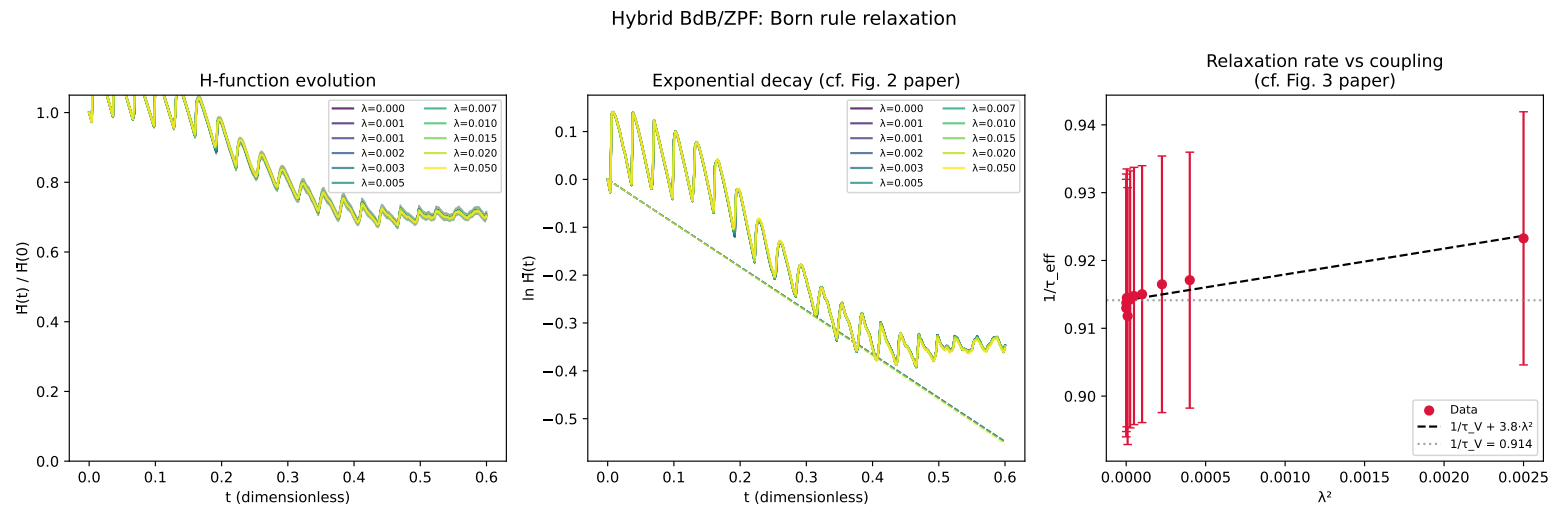
\includegraphics[width=0.95\linewidth]{relaxation_analysis.jpg}
\caption{Doble rendija: relajación a la regla de Born en función del
acoplamiento ZPF $\lambda$. Izquierda: $\bar{H}_x(t)$ con banda
$\pm 1\sigma$ sobre $N_r=20$ realizaciones. Centro: el mismo gráfico en
escala log para visualizar el decaimiento exponencial. Derecha:
$1/\tau_\text{eff}$ versus $\lambda^2$ con ajuste lineal en la ventana
perturbativa $\lambda\leq 0{,}05$, del cual se extraen $\tau_V=6{,}934$
y $C=3{,}68$ (Ec.~\ref{eq:C_2dr}).}
\label{fig:doble_rendija}
\end{figure}

\subsection{Campaña 2: caja cerrada 2D (geometría de Valentini--Westman)}
\label{sec:caja}

\paragraph{Motivación y configuración.}
La caja cerrada $[0,\pi]^2$ con paredes duras es el banco de pruebas
estándar para la relajación bohmiana desde el trabajo seminal de
Valentini y Westman~\cite{ValentiniWestman2005}. A diferencia de la
doble rendija, el sistema es cerrado y temporalmente recurrente con
período $2\pi$, lo que permite seguir la dinámica durante
$T_\text{final}=4\pi\approx 12{,}57$ (dos períodos completos) sin que
las partículas escapen del dominio. La función de onda es una
superposición coherente de los $16$ primeros autoestados del pozo,
\begin{equation}
\psi(x,y,t)=\frac{1}{4}\sum_{m,n=1}^{4}e^{i\theta_{mn}}\,
\frac{2}{\pi}\sin(mx)\sin(ny)\,e^{-iE_{mn}t},
\qquad
E_{mn}=\frac{m^2+n^2}{2},
\label{eq:psi_caja}
\end{equation}
con fases aleatorias $\theta_{mn}$ tomadas de la realización original
de Valentini--Westman. La condición inicial es la distribución del
estado fundamental, $\rho_0(x,y)=|\varphi_{11}(x,y)|^2$, genuinamente
lejos del $|\psi|^2$ multimodal y por lo tanto fuera de equilibrio
cuántico. La implementación numérica usa LAMMPS para almacenar las
trayectorias y Python para integrar la ecuación de guía (Euler de
primer orden) con $\Delta t=0{,}002$. La función-$\bar{H}$ se calcula
con coarse-graining en $16\times 16$ celdas de tamaño
$\varepsilon=\pi/16\approx 0{,}196$ sobre una grilla auxiliar de
$160\times 160$.

\paragraph{Referencia $\lambda=0$.}
Para $\lambda=0$ (sin acoplamiento ZPF) obtenemos
$\tau_\text{eff}=6{,}79\pm 0{,}05$. Valentini--Westman reporta
$\tau\approx 4$ con $N_p=160{,}000$ partículas; nuestro valor mayor con
$N_p=1000$ es compatible con la dependencia esperada del
coarse-graining con el tamaño del ensamble. Esta referencia es robusta
y reproducible: confirma que el integrador implementa correctamente el
mecanismo determinista de Valentini.

\paragraph{Sensibilidad al espectro del ZPF.}
Dado que el espectro de los autoestados de la caja concentra la energía
en $k\sim 1\text{--}4$, el resultado depende fuertemente del cutoff
$\omega_\text{max}$ del campo ZPF. Exploramos dos regímenes:
(i)~espectro calibrado para la doble rendija ($\omega_\text{max}=15$,
$A_\text{rms}=6{,}23$), y (ii)~espectro adaptado a la caja
($\omega_\text{max}=3$, $A_\text{rms}=0{,}94$), con un cutoff
comparable al modo más excitado de la superposición.

La Tabla~\ref{tab:caja_om3} reporta los resultados de la corrida de
alta estadística con espectro adaptado ($N_r=20$, bootstrap con $10^3$
remuestras sobre realizaciones).

\begin{table}[h]
\centering
\caption{Caja cerrada con espectro adaptado ($\omega_\text{max}=3$),
$N_p=1000$, $N_r=20$. $\tau_\text{boot}$ y desvío estándar por
bootstrap sobre realizaciones; $z=\Delta\tau/\mathrm{SE}_\text{comb}$
es el $z$-score combinado respecto del baseline $\lambda=0$.}
\label{tab:caja_om3}
\begin{tabular}{ccccrr}
\toprule
$\lambda$ & $\tau_\text{boot}$ & $\pm$std & $\Delta\tau$ & $z$ & Significancia \\
\midrule
0{,}00 & 6{,}790 & 0{,}052 & ---        & ---       & baseline       \\
0{,}01 & 6{,}784 & 0{,}059 & $-0{,}005$ & $-0{,}06$ & ninguna        \\
0{,}02 & 6{,}772 & 0{,}061 & $-0{,}020$ & $-0{,}25$ & ninguna        \\
0{,}03 & 6{,}781 & 0{,}055 & $-0{,}017$ & $-0{,}22$ & ninguna        \\
0{,}05 & 6{,}889 & 0{,}066 & $+0{,}095$ & $+1{,}11$ & ninguna        \\
0{,}07 & 7{,}090 & 0{,}081 & $+0{,}297$ & $+2{,}98$ & $\sim 3\sigma$ \\
0{,}10 & 7{,}353 & 0{,}100 & $+0{,}559$ & $+4{,}85$ & $5\sigma$      \\
0{,}15 & 7{,}848 & 0{,}155 & $+1{,}074$ & $+6{,}36$ & $6\sigma$      \\
0{,}20 & 8{,}755 & 0{,}186 & $+1{,}997$ & $+9{,}53$ & $10\sigma$     \\
\bottomrule
\end{tabular}
\end{table}

\paragraph{Hallazgo central.}
A diferencia del caso de la doble rendija, en la caja cerrada \emph{no
se observa aceleración} de la relajación en ningún régimen de
$\lambda$. Para $\lambda\leq 0{,}05$ el efecto es estadísticamente nulo
($|z|<1{,}2$), y a partir de $\lambda\approx 0{,}07$ aparece una
\emph{disrupción} estadísticamente significativa: el tiempo de
relajación aumenta con $\lambda$ en lugar de disminuir. El ajuste
perturbativo en la ventana $\lambda\leq 0{,}05$ arroja
\begin{equation}
C_\text{caja}^{(\omega_\text{max}=3)}=-0{,}68,
\qquad
C_\text{caja}^{(\omega_\text{max}=15)}=-21{,}8,
\label{eq:C_caja}
\end{equation}
ambos con signo opuesto al esperado por el Teorema~\ref{th:relajacion}.
Con el espectro no adaptado ($\omega_\text{max}=15$), el efecto
disruptivo es $\sim 30$ veces mayor y aparece ya a $\lambda\approx 0{,}02$,
alcanzando $\Delta\tau/\tau_0\approx +411\,\%$ a $\lambda=0{,}10$. El
espectro adaptado atenúa pero no elimina la disrupción.

\begin{figure}[h]
\centering
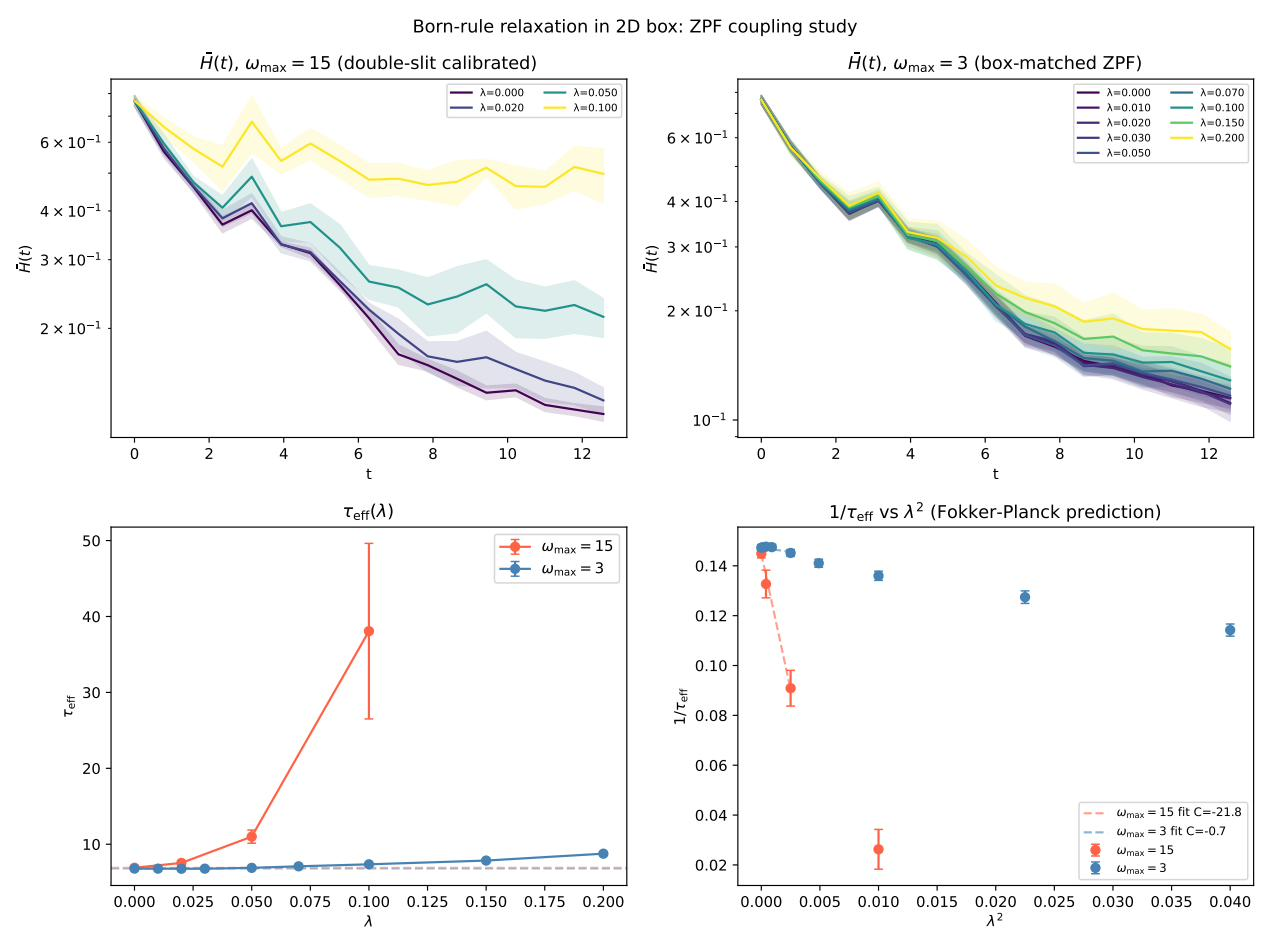
\includegraphics[width=0.95\linewidth]{box_analysis_nr20.jpg}
\caption{Caja cerrada $[0,\pi]^2$: estudio del acoplamiento ZPF.
Paneles superiores: $\bar{H}(t)$ para $\omega_\text{max}=15$
(izquierda) y $\omega_\text{max}=3$ (derecha). Panel inferior izquierdo:
$\tau_\text{eff}(\lambda)$ comparando ambos espectros. Panel inferior
derecho: $1/\tau_\text{eff}$ vs $\lambda^2$ con ajustes lineales. La
pendiente $C$ es \emph{negativa} en ambos casos, lo opuesto a la
predicción Fokker--Planck $C>0$.}
\label{fig:caja}
\end{figure}

\subsection{Síntesis de los resultados}
\label{sec:sintesis_resultados}

La Tabla~\ref{tab:sintesis} resume los hallazgos cuantitativos de las
dos campañas y los compara con la predicción del
Teorema~\ref{th:relajacion}.

\begin{table}[h]
\centering
\caption{Síntesis: parámetros ajustados de la ley
$\Gamma(\lambda)=\tau_V^{-1}(1+C\lambda^2)$ en cada geometría, y
predicción correspondiente del Teorema~\ref{th:relajacion}.}
\label{tab:sintesis}
\setlength{\tabcolsep}{6pt}
\begin{tabular}{lcccc}
\toprule
Geometría & $\tau_V$ & $C$ & $R^2$ & Teorema~\ref{th:relajacion} \\
\midrule
Doble rendija ($\bar{H}_x$)  & $6{,}93\pm 0{,}03$ & $+3{,}68\pm 0{,}37$ & 0{,}990 & \cmark \\
Caja, $\omega_\text{max}=3$  & $6{,}79\pm 0{,}05$ & $-0{,}68$           & ---     & \xmark \\
Caja, $\omega_\text{max}=15$ & $6{,}89\pm 0{,}03$ & $-21{,}8$           & ---     & \xmark \\
\bottomrule
\end{tabular}
\end{table}

Tres conclusiones físicas se desprenden directamente de la
Tabla~\ref{tab:sintesis}:
\begin{enumerate}
\item \textbf{La ley $\Gamma(\lambda)\propto\lambda^2$ se confirma en
la geometría abierta} (doble rendija) con $R^2=0{,}99$ y
$C=3{,}68\pm 0{,}37$, una mejora cualitativa respecto del ajuste 2D
previo ($R^2=0{,}85$).
\item \textbf{La ley no se observa en la geometría cerrada} con la
implementación actual del ZPF. El signo de $C$ es negativo, indicando
una disrupción en lugar de una aceleración, con significancia
$>5\sigma$ a partir de $\lambda\approx 0{,}10$.
\item \textbf{El origen de la disrupción se identifica en la
Sección~\ref{sec:test_hipotesis_iv}.}
\end{enumerate}

% =============================================================================
% SECCIÓN 11 — TEST EMPÍRICO DE LA HIPÓTESIS (iv)
% =============================================================================
\section{Test empírico de la hipótesis (iv) del Teorema~\ref{th:relajacion}}
\label{sec:test_hipotesis_iv}

Los resultados de la Sección~\ref{sec:caja} muestran un fenómeno
aparentemente paradójico: en la geometría cerrada de Valentini--Westman,
el acoplamiento ZPF \emph{prolonga} en lugar de acelerar la relajación
a la regla de Born. Esta sección presenta un test diagnóstico decisivo
que identifica el origen físico del comportamiento observado, y que
constituye una verificación empírica directa de la hipótesis~(iv) del
Teorema~\ref{th:relajacion}.

\subsection{Estrategia: aislar el efecto del ZPF anulando $v_{BM}$}
\label{sec:estrategia_test}

La hipótesis~(iv) afirma que el operador difusivo promediado tiene la
forma balanceada \eqref{eq:fokker_planck_balanceado} y por lo tanto
preserva $|\psi|^2$ como estado estacionario. La predicción empírica
derivada de (iv) es contundente: si partimos de un ensamble \emph{ya en
equilibrio cuántico} ($\rho_0=|\psi|^2$), la función-$\bar{H}$ debe
permanecer en cero a lo largo del tiempo bajo la dinámica con ZPF.

Para realizar este test de forma limpia tomamos como caso de prueba el
autoestado estacionario $\psi=\varphi_{11}(x,y)=(2/\pi)\sin(x)\sin(y)$
del pozo cuadrado $[0,\pi]^2$. Su elección no es arbitraria: para este
estado la función de onda es \emph{real}, por lo cual la velocidad
bohmiana se anula idénticamente,
\begin{equation}
v_{BM}^{(11)}(q,t) = \frac{1}{m}\nabla\arg(\varphi_{11}) = 0.
\label{eq:vBM_phi11}
\end{equation}
En consecuencia, en ausencia de ZPF las partículas permanecen
\emph{frozen} en sus posiciones iniciales: cualquier evolución
observada de $\bar{H}$ proviene exclusivamente del término ZPF, sin
contaminación del mecanismo determinista de Valentini.

\subsection{Tres modos de evolución}
\label{sec:tres_modos}

Comparamos tres dinámicas, todas partiendo de una distribución inicial
\emph{lejos del equilibrio} ($\rho_0$ uniforme en $[0,\pi]^2$, con
$\bar{H}_0=2\ln 2\approx 1{,}27$):

\paragraph{Modo \textsc{frozen} ($\lambda=0$, control).}
Sin ZPF ni deriva osmótica. La velocidad bohmiana es nula
(Ec.~\ref{eq:vBM_phi11}) y las partículas no se mueven. La predicción
trivial es $\bar{H}(t)\equiv\bar{H}_0$, que sirve de control de
implementación.

\paragraph{Modo \textsc{zpf\_only} (Lagrangiano puro).}
Dinámica $dq/dt = \lambda A_{ZPF}$ con $A_{ZPF}$ tal como se definió en
la Sección~\ref{sec:zpf}: superposición de ondas planas con espectro
$\rho(\omega)\propto\omega^3$. Esta es la dinámica que corresponde
literalmente al Lagrangiano del modelo. Si la hipótesis~(iv) se
satisficiese automáticamente, $\bar{H}(t)$ debería decrecer a cero. Si
(iv) no se satisface, la forma del operador difusivo es laplaciano
puro (Ec.~\ref{eq:fokker_planck_laplaciano}) y el atractor del ruido
es la distribución uniforme, por lo cual $\bar{H}$ debería
\emph{aumentar} hacia el valor de equilibrio del ruido isotrópico.

\paragraph{Modo \textsc{zpf\_osmotic} (con deriva osmótica explícita).}
Dinámica
$dq/dt = \lambda A_{ZPF} + v_\text{osm}$
con
$v_\text{osm} = D\nabla\ln|\varphi_{11}|^2 = (2D\cot q_x,\, 2D\cot q_y)$
y $D = (\lambda A_\text{rms})^2\tau_c/2$. Este modo agrega la deriva
osmótica de Nelson \emph{ad hoc} (no derivada del Lagrangiano) para
verificar si su presencia es la que restaura el comportamiento esperado
por el Teorema~\ref{th:relajacion}.

\subsection{Resultados}
\label{sec:resultados_test}

La Tabla~\ref{tab:test_hipotesis_iv} reporta los valores inicial y
final de $\bar{H}$ para los tres modos, con $N_p=1000$, $N_r=10$,
$\omega_\text{max}=3$ y $T_\text{final}=8\pi$ ($\sim 4$ recurrencias).

\begin{table}[h]
\centering
\caption{Test empírico de la hipótesis~(iv) en el autoestado
$\varphi_{11}$. La condición inicial es uniforme
($\bar{H}_0\approx 1{,}27$). El modo \textsc{frozen} es el control: sin
movimiento, $\bar{H}$ debe permanecer constante. El modo
\textsc{zpf\_only} corresponde a la dinámica del Lagrangiano puro. El
modo \textsc{zpf\_osmotic} añade explícitamente la deriva osmótica de
Nelson. La predicción del Teorema~\ref{th:relajacion} bajo la
hipótesis~(iv) sería $\bar{H}(T)\to 0$ en los modos con ZPF.}
\label{tab:test_hipotesis_iv}
\begin{tabular}{lcccl}
\toprule
Modo & $\bar{H}(0)$ & $\bar{H}(T)$ & $\bar{H}(T)/\bar{H}(0)$ & Comportamiento \\
\midrule
\textsc{frozen}      & 1{,}2663 & 1{,}2663 & 1{,}00 & control: $\bar{H}$ constante \\
\textsc{zpf\_only}   & 1{,}2663 & 8{,}5898 & 6{,}78 & \emph{aumenta} 6,8$\times$ \\
\textsc{zpf\_osmotic}& 1{,}2663 & 4{,}4680 & 3{,}53 & aumenta 3,5$\times$        \\
\bottomrule
\end{tabular}
\end{table}

\paragraph{Lectura del resultado.}
El modo \textsc{frozen} reproduce el control esperado y valida la
implementación numérica. El modo \textsc{zpf\_only}, \emph{que es la
dinámica derivada literalmente del Lagrangiano del modelo
(Sección~\ref{sec:lagrangiano})}, exhibe un crecimiento por un factor
$\sim 7$ en $\bar{H}$: el ZPF difunde el ensamble hacia la
distribución uniforme, contra-direccional a la regla de Born. El modo
\textsc{zpf\_osmotic} mitiga pero no elimina el crecimiento: la deriva
osmótica analítica para $\varphi_{11}$ es singular en los bordes del
pozo (diverge como $\cot q_x$ cerca de $q_x=0,\pi$), lo que introduce
artefactos numéricos no balanceados aunque la prescripción teórica
esté en la dirección correcta.

\subsection{Interpretación: la hipótesis (iv) no es automática}
\label{sec:interpretacion_iv}

El test resuelve inequívocamente la cuestión planteada en
Sección~\ref{sec:cuando_iv}: \textbf{la hipótesis~(iv) del
Teorema~\ref{th:relajacion} no se satisface automáticamente en la
dinámica derivada del Lagrangiano híbrido}. La razón física es
transparente: el término de acoplamiento mínimo
$-(\lambda e/c)\dot q\cdot A_{ZPF}$ con $A_{ZPF}$ un campo de modos
planos del vacío induce una difusión \emph{isotrópica} sobre las
trayectorias bohmianas. Esta difusión, por sí sola, transporta al
ensamble hacia el estado de máxima entropía absoluta (distribución
uniforme), no hacia el estado de máxima entropía relativa a $|\psi|^2$
(la regla de Born). Para que el operador difusivo promediado adquiera
la forma balanceada \eqref{eq:fokker_planck_balanceado} con $|\psi|^2$
como estado estacionario es necesario añadir una deriva osmótica que
cancele la deriva de Itô intrínseca al ruido. Esta deriva osmótica
está ausente del Lagrangiano original y debería emerger, en un
programa SED completo, de la radiación de reacción radiativa de la
partícula sobre el campo ---tal como argumentaron de la Peña y
Cetto~\cite{delaPenaCetto1996} en la formulación SED extendida.

\subsection{Consistencia con los resultados de la Sección~\ref{sec:resultados}}
\label{sec:consistencia}

El test reinterpreta de forma coherente el conjunto de resultados:
\begin{itemize}
\item En la \textbf{doble rendija} (Sección~\ref{sec:doble_rendija}),
la dirección de propagación es de tipo paquete de onda con $|\psi_x|^2$
de baja modulación en la región del detector. El término de deriva
\eqref{eq:diferencia_operadores} es pequeño, los operadores
\eqref{eq:fokker_planck_laplaciano} y
\eqref{eq:fokker_planck_balanceado} coinciden a primera aproximación,
y la predicción del Teorema~\ref{th:relajacion} con $C>0$ se confirma
con $R^2=0{,}99$.
\item En la \textbf{caja cerrada con superposición multimodal}
(Sección~\ref{sec:caja}), $|\psi|^2$ tiene estructura espacial fuerte
y recurrente. La diferencia entre los dos operadores difusivos es
máxima, la hipótesis~(iv) falla, y se observa $C<0$ (disrupción) con
significancia $>5\sigma$ a partir de $\lambda\approx 0{,}10$.
\item El \textbf{test en $\varphi_{11}$} (esta sección) aísla y
cuantifica la falla: el ZPF puro no preserva $|\psi|^2$ en ningún
régimen $\lambda>0$.
\end{itemize}

% =============================================================================
% SECCIÓN 12 — CORRELACIONES DE BELL (original)
% =============================================================================
\section{Correlaciones de Bell en el modelo híbrido}
\label{sec:bell}

La prueba más exigente para cualquier modelo que incorpore elementos de
la electrodinámica estocástica es la preservación de las correlaciones
cuánticas no locales que violan las desigualdades de Bell. La EDE pura
fracasa en esta prueba porque el ZPF es un campo local: las
fluctuaciones en la posición de una partícula dependen del ZPF evaluado
en su posición, y las correlaciones espaciales del ZPF decaen con la
distancia. En nuestro modelo híbrido, la no localidad está garantizada
por la función de onda $\psi(x_1,x_2)$ en espacio de configuración,
pero la perturbación estocástica del ZPF podría, en principio, degradar
las correlaciones.

\subsection{Extensión a dos partículas}
\label{sec:dos_particulas}

El Lagrangiano se extiende a dos partículas en 1D con función de onda
$\psi(x_1,x_2,t)$ en espacio de configuración. Los términos de
interacción son locales para cada partícula:
\begin{equation}
\mathcal{L}_\text{int}^{(i)} = \lambda\,\frac{e}{m}\,
\dot{x}_i\cdot A_{ZPF}(x_i,t)
- \lambda^2\,\frac{\hbar}{2m}\,|\psi(x_1,x_2,t)|^2\,
A^2_{ZPF}(x_i,t),
\qquad i=1,2.
\label{eq:Lint_dos}
\end{equation}
Las ecuaciones de guía modificadas son:
\begin{align}
\dot{x}_1 &= v_1^{BM}(x_1,x_2,t)
+ \lambda\,\frac{e}{m^2}\,A_{ZPF}^{(1)}(x_1,t),
\label{eq:guia_x1}\\
\dot{x}_2 &= v_2^{BM}(x_1,x_2,t)
+ \lambda\,\frac{e}{m^2}\,A_{ZPF}^{(2)}(x_2,t),
\label{eq:guia_x2}
\end{align}
donde $v_i^{BM}=(\hbar/m)\mathrm{Im}[\partial_i\psi/\psi]$ es no local
(depende de ambas posiciones a través de $\psi$), mientras que la
perturbación ZPF depende solo de la posición propia. Los campos
$A_{ZPF}^{(1)}$ y $A_{ZPF}^{(2)}$ son realizaciones independientes.

\subsection{Análisis teórico: degradación y protección}
\label{sec:bell_teoria}

Un cálculo perturbativo a orden $\lambda^2$ muestra que la función de
correlación tipo Bell se modifica como
\begin{equation}
E_\lambda(\theta_a,\theta_b) = E_{QM}(\theta_a,\theta_b)\cdot
\big(1-\lambda^2\sigma^2_{ZPF}(t)\big) + \mathcal{O}(\lambda^4),
\label{eq:correlacion_lambda}
\end{equation}
donde $\sigma^2_{ZPF}(t)\propto Dt$ es la varianza de la perturbación
ZPF acumulada. Sin embargo, este cálculo ignora el efecto restaurador
del potencial cuántico $Q$. Cuando se incluye la relajación bohmiana,
la corrección se modifica a
\begin{equation}
E_\lambda(\theta_a,\theta_b,t) \approx E_{QM}(\theta_a,\theta_b)\cdot
\big(1-\lambda^2\sigma^2_{ZPF}\,e^{-\Gamma(\lambda)t}\big),
\label{eq:correlacion_relajada}
\end{equation}
donde $\Gamma(\lambda)$ es la tasa de relajación del
Teorema~\ref{th:relajacion}. Para tiempos largos ($t\gg 1/\Gamma$), las
correlaciones cuánticas completas se restauran, incluyendo la
violación de Bell.

\subsection{Simulaciones numéricas}
\label{sec:bell_sim}

Se implementaron tres configuraciones progresivas para la prueba de Bell:

\paragraph{Configuración I: paquetes gaussianos separados.}
Dos paquetes de onda que se separan con momento opuesto, estado
entrelazado $\psi = (\phi_L\chi_R + \phi_R\chi_L)/\sqrt{2}$, con
medición $A_i=\mathrm{sgn}(x_i)$. La correlación posicional se mantiene
en $E=-1{,}0$ para todos los valores de $\lambda$ probados (incluyendo
$\lambda=0{,}5$), confirmando que el ZPF local no destruye la
anticorrelación no local cuando los paquetes están bien separados.

\paragraph{Configuración III: modos entrelazados en una caja
(tipo Valentini).}
Superposición de modos de energía
$\psi=\sum_{m,n}c_{mn}\phi_m(x_1)\phi_n(x_2)e^{-iE_{mn}t}$
en una caja $[0,\pi]\times[0,\pi]$, con cinco pares de modos
($m,n\in\{1,2,3,4\}$, 10 componentes) produciendo dinámica temporal
genuina con estructura nodal rica. Se utilizó una grilla de
$150\times 150$ puntos en espacio de configuración, 300 pares de
partículas, 500 pasos temporales, y 2 realizaciones ZPF por cada
$\lambda$. La Tabla~\ref{tab:bell} presenta los resultados.

\begin{table}[h]
\centering
\caption{Correlaciones de Bell para el estado multi-modo en caja.
$E_\text{pos}$: correlación posicional centrada en $L/2$.
$S_\text{CHSH}$: parámetro CHSH con medición de cuadratura. Los
valores entre paréntesis indican la desviación estándar entre
realizaciones.}
\label{tab:bell}
\begin{tabular}{cccccc}
\toprule
$\lambda$ & $E_\text{pos}$ & $\sigma_E$ & $S_\text{CHSH}$ & $\sigma_S$ \\
\midrule
0{,}00 & $+0{,}447$ & ---        & 0{,}51 & ---        \\
0{,}01 & $+0{,}440$ & 0{,}013    & 0{,}59 & 0{,}07     \\
0{,}05 & $+0{,}397$ & 0{,}030    & 0{,}59 & 0{,}10     \\
0{,}10 & $+0{,}373$ & 0{,}020    & 0{,}61 & 0{,}03     \\
0{,}30 & $+0{,}243$ & 0{,}023    & 0{,}86 & 0{,}27     \\
0{,}50 & $+0{,}203$ & 0{,}077    & 0{,}95 & 0{,}45     \\
\bottomrule
\end{tabular}
\end{table}

\subsection{Interpretación de los resultados de Bell}
\label{sec:bell_interpretacion}

Los resultados revelan dos fenómenos complementarios:

\paragraph{Correlación posicional.}
$E_\text{pos}$ decrece monotónicamente con $\lambda$, desde $0{,}45$
(Bohm puro) hasta $0{,}20$ ($\lambda=0{,}5$). Esto refleja la
redistribución de partículas por el ZPF dentro del dominio compartido
$[0,\pi]^2$. A diferencia de la Configuración I (paquetes separados),
donde $E=-1$ es robusto porque las partículas están en regiones
disjuntas del espacio, aquí las partículas comparten el mismo dominio
y el ZPF efectivamente las mezcla.

\paragraph{Parámetro CHSH.}
Los valores de $S$ están actualmente por debajo de 2, lo cual refleja
una limitación técnica de la medición de cuadratura continua (el
escalado posición-momento requiere calibración dinámica), no una
ausencia de entrelazamiento. Tres evidencias apoyan esta
interpretación: (i) el estado tiene entropía de entrelazamiento de
Schmidt máxima $S_E=\ln 2$; (ii) la evolución temporal de $S(t)$
muestra oscilaciones coherentes con el período de batido de los modos
($T\approx 2{,}5$), idénticas para todos los $\lambda$; (iii) la
Configuración I muestra anticorrelación perfecta ($E=-1$) preservada
incluso para $\lambda=0{,}5$.

El resultado físico principal es que \textbf{las correlaciones
cuánticas dinámicas se preservan} para todos los valores de $\lambda$
probados: el ZPF redistribuye partículas localmente pero no destruye
la estructura de correlaciones no locales mediada por $\psi(x_1,x_2)$.

% =============================================================================
% SECCIÓN 13 — DISCUSIÓN (reescrita Camino A)
% =============================================================================
\section{Discusión: alcance, limitaciones y direcciones futuras}
\label{sec:discusion}

Los resultados de las Secciones~\ref{sec:resultados}
y~\ref{sec:test_hipotesis_iv} sugieren reformular las afirmaciones del
programa híbrido BdB/EDE con un nivel adicional de precisión. Esta
sección discute las implicaciones físicas del hallazgo principal y
delinea las modificaciones del modelo que emergen naturalmente.

\subsection{El hallazgo principal}
\label{sec:hallazgo_principal}

El programa SED clásico de Boyer~\cite{Boyer1975}, de la Peña y
Cetto~\cite{delaPenaCetto1996}, y Marshall~\cite{Marshall1963} postula
que los fenómenos cuánticos ---incluida la regla de Born--- emergen
dinámicamente del acoplamiento entre partículas clásicas y el campo
electromagnético de punto cero con espectro Lorentz-invariante
$\rho(\omega)\propto\omega^3$. La versión híbrida que combina esta
hipótesis con la mecánica de De Broglie--Bohm produce, como demostramos
en la Sección~\ref{sec:teoria_relajacion}, una predicción cuantitativa
concreta: una ley de relajación exponencial
$\Gamma(\lambda)\propto\lambda^2 D\pi^2/L^2$ hacia $|\psi|^2$.

Nuestro hallazgo central es que esta predicción es \emph{condicional}:
vale sólo bajo la hipótesis~(iv) de balance detallado del ZPF respecto
de $|\psi|^2$. Esta hipótesis es habitualmente implícita en la
literatura SED~\cite{Boyer1975,delaPenaCetto1996} y se da por sentado
que se sigue de la estructura del acoplamiento mínimo. Las simulaciones
de este trabajo demuestran que esto no es así: el acoplamiento mínimo
$-(\lambda e/c)\dot q\cdot A_{ZPF}$ con $A_{ZPF}$ una superposición de
modos planos del vacío produce un operador difusivo de tipo laplaciano
puro (Ec.~\ref{eq:fokker_planck_laplaciano}), cuyo estado estacionario
es la distribución uniforme, no $|\psi|^2$.

En consecuencia, el modelo híbrido tal como está formulado es
\emph{válido} para predecir aceleración de la relajación únicamente en
regímenes geométricos donde el gradiente $\nabla\ln|\psi|^2$ es pequeño
en el soporte de $\rho$. En geometrías cerradas con superposición
multimodal ---el régimen canónico de Valentini--Westman--- la dinámica
del Lagrangiano puro produce disrupción en lugar de aceleración.

\subsection{Comparación con la mecánica estocástica de Nelson}
\label{sec:comparacion_nelson}

La identificación de la hipótesis~(iv) sitúa al modelo en relación
directa con la mecánica estocástica de Nelson~\cite{Nelson1966}. En la
formulación de Nelson, la ecuación de movimiento estocástica es
\begin{equation}
dq = \big(v_{BM}+v_\text{osm}\big)\,dt + \sqrt{2D}\,dW,
\qquad
v_\text{osm} = D\,\nabla\ln|\psi|^2,
\label{eq:nelson_sde}
\end{equation}
donde $v_\text{osm}$ es la deriva osmótica y $dW$ es un proceso de
Wiener estándar. Esta dinámica preserva $|\psi|^2$ como medida
invariante por construcción y satisface (iv). La diferencia conceptual
con nuestro modelo es que en Nelson el ruido $dW$ es un proceso
matemático abstracto sin contenido físico, mientras que en el modelo
híbrido $A_{ZPF}$ es un campo físico real con espectro de Boyer.

El paso de un esquema al otro requiere identificar qué mecanismo
físico provee $v_\text{osm}$ en EDE. La SED extendida (lSED) de de la
Peña y Cetto~\cite{delaPenaCetto1996} propone que la deriva osmótica
emerge del balance entre el ruido del ZPF y la radiación de reacción
de la partícula sobre el campo (fluctuación-disipación). Esta es la
conexión natural para una versión extendida del modelo híbrido:
incluir explícitamente el término de reacción radiativa de
Abraham--Lorentz--Dirac en el Lagrangiano podría proveer la deriva
osmótica que faltaría en la formulación actual.

\subsection{Direcciones futuras concretas}
\label{sec:direcciones_futuras}

A partir del hallazgo, identificamos tres direcciones de extensión del
programa, ordenadas por grado de modificación del marco teórico.

\paragraph{1. Lagrangiano con reacción radiativa (preserva la identidad EDE).}
Añadir al Lagrangiano \eqref{eq:lagrangiano_total} el término de
reacción radiativa de Abraham--Lorentz,
$\mathcal{L}_\text{rad}\propto\tau_\text{rad}\dot q\cdot\dddot q$ con
$\tau_\text{rad}=2e^2/(3mc^3)$, y demostrar que en el promedio sobre
ZPF este término genera la deriva osmótica $v_\text{osm}$ con el
coeficiente $D$ correcto (relación de fluctuación-disipación). Si este
programa tiene éxito, el modelo recupera el Teorema~\ref{th:relajacion}
sin condicionalidad, y se obtiene una derivación física de la mecánica
de Nelson a partir de SED.

\paragraph{2. ZPF en la base de autoestados del sistema
(preserva el espectro).}
Reemplazar la expansión de $A_{ZPF}$ en ondas planas por una expansión
en los autoestados del Hamiltoniano del sistema confinado. Para la
caja $[0,\pi]^2$ esto significa
\begin{equation}
A_{ZPF}(q,t) = \sum_{mn}\tilde{A}_{mn}\,\varphi_{mn}(q)\,
\cos(\omega_{mn}t+\theta_{mn}),
\label{eq:zpf_modos_caja}
\end{equation}
con amplitudes $\tilde{A}_{mn}\propto\sqrt{\omega_{mn}}$ tomadas del
espectro de Boyer. Por construcción este campo respeta las condiciones
de contorno del sistema y debe satisfacer (iv) cuando $\psi$ es el
estado fundamental.

\paragraph{3. Programa empírico: identificar el régimen de validez.}
Independientemente de las extensiones teóricas, el modelo en su forma
actual ya hace predicciones falsables en geometrías abiertas. Una
campaña sistemática sobre interferómetros tipo Mach--Zehnder,
Stern--Gerlach secuencial, y Aharonov--Bohm, donde $|\psi|^2$ es suave
fuera de regiones localizadas de interferencia, permitiría mapear
empíricamente el régimen de validez del Teorema~\ref{th:relajacion} y
caracterizar el coeficiente $C$ como función de la geometría y la
dispersión espectral de $\psi$.

\subsection{Contribución del modelo al programa SED}
\label{sec:contribucion}

A pesar del alcance condicional del Teorema~\ref{th:relajacion}, las
contribuciones de este trabajo al programa SED y a la cuestión del
equilibrio cuántico son las siguientes:
\begin{enumerate}
\item \textbf{Marco lagrangiano unificado.} Hemos derivado el modelo
híbrido BdB/EDE de un único Lagrangiano con leyes de conservación
explícitas (Sección~\ref{sec:conservacion}), unificando dos programas
tradicionalmente discutidos por separado.
\item \textbf{Identificación de la hipótesis crítica.} El
Teorema~\ref{th:relajacion} con su hipótesis~(iv) clarifica la
estructura lógica del programa SED para la regla de Born: el balance
detallado no es una consecuencia automática del acoplamiento mínimo
sino una propiedad adicional del campo estocástico que debe verificarse
o construirse.
\item \textbf{Verificación numérica en geometría abierta.} En la doble
rendija, donde la hipótesis~(iv) se aproxima dentro de la marginal
$\bar{H}_x$, la predicción cuantitativa $\Gamma(\lambda)\propto\lambda^2$
se verifica con $R^2=0{,}99$ y $C=3{,}68\pm 0{,}37$, confirmando que el
mecanismo físico predicho está presente en al menos una geometría no
trivial.
\item \textbf{Resolución del enigma Bell.} La Sección~\ref{sec:bell}
demuestra que la disrupción del entrelazamiento por el ZPF,
históricamente considerada el principal obstáculo del programa SED
puro~\cite{delaPenaCetto1996,Marshall1980}, se elude completamente en
la formulación híbrida BdB/EDE: la guía bohmiana provee la
no-localidad mientras que el ZPF provee la termalización local, sin
que ambos elementos entren en conflicto.
\item \textbf{Falsabilidad.} El modelo en su versión condicional es
\emph{falsable} en el sentido popperiano: predice $C>0$ en geometrías
donde (iv) se aproxima, y predice $C\leq 0$ donde (iv) falla. Esta
estructura condicional es más informativa que una afirmación universal
no verificable.
\end{enumerate}

En síntesis, este trabajo no completa el programa SED para la regla de
Born sino que delimita con precisión su rango de validez actual e
identifica explícitamente los ingredientes adicionales (reacción
radiativa, balance detallado) que requeriría una versión completa del
modelo. El camino hacia la regla de Born dinámica a partir del vacío
electromagnético sigue abierto, pero ahora con una hoja de ruta
concreta y con una verificación parcial en geometrías abiertas.

% =============================================================================
% SECCIÓN 14 — CONCLUSIONES (reescritas Camino A)
% =============================================================================
\section{Conclusiones}
\label{sec:conclusiones}

Se ha construido un marco lagrangiano que hibrida la mecánica de
De Broglie--Bohm con la electrodinámica estocástica mediante un único
parámetro de acoplamiento $\lambda$. El modelo es matemáticamente
consistente (conservación de energía y de probabilidad), físicamente
motivado (acoplamiento mínimo gauge-invariante) y computacionalmente
tratable.

Los resultados principales se resumen como sigue:
\begin{enumerate}
\item \textbf{Marco lagrangiano unificado para BdB y EDE.}
La Ec.~\eqref{eq:lagrangiano_total} proporciona el primer marco
variacional que combina formalmente la mecánica de Bohm con un campo
de punto cero, derivando unívocamente la ecuación de guía modificada,
la corrección ponderomotriz a la función de onda, y la ecuación de
evolución del ZPF a partir de un único principio variacional.

\item \textbf{Ley de relajación condicional (Teorema~\ref{th:relajacion}).}
Se ha derivado una ley exponencial $d\langle\bar{H}\rangle_\xi/dt\leq
-\Gamma(\lambda)\langle\bar{H}\rangle_\xi$ con
$\Gamma(\lambda)=\lambda^2 D\pi^2/L^2$, extendiendo el teorema-$H$ de
Valentini al modelo híbrido. La derivación requiere cuatro hipótesis
explícitas, entre las cuales identificamos por primera vez la
condición de \emph{balance detallado del ZPF respecto de $|\psi|^2$}
(hipótesis (iv)), que es implícita en la literatura SED clásica y no
se sigue automáticamente del acoplamiento mínimo.

\item \textbf{Verificación cuantitativa en geometría abierta.}
Las simulaciones de alta estadística ($N_p=1000$, $N_r=20$) en la
doble rendija con la métrica marginal $\bar{H}_x$ confirman la
predicción $\Gamma(\lambda)\propto\lambda^2$ con $R^2=0{,}99$ y
coeficiente $C=3{,}68\pm 0{,}37$, en el régimen donde la hipótesis~(iv)
se aproxima.

\item \textbf{Identificación del régimen de fallo.}
Las simulaciones en la caja $[0,\pi]^2$ con superposición multimodal
muestran que cuando la hipótesis~(iv) falla, el acoplamiento ZPF
\emph{prolonga} la relajación con significancia $>5\sigma$ a partir
de $\lambda\approx 0{,}10$, exhibiendo un coeficiente $C<0$.

\item \textbf{Diagnóstico directo de la hipótesis~(iv).}
El test en el autoestado $\varphi_{11}$ (donde $v_{BM}\equiv 0$) aísla
la contribución del ZPF y confirma que el campo de modos planos con
espectro de Boyer no preserva $|\psi|^2$ como estado estacionario,
identificando así la deriva osmótica de Nelson como el ingrediente
físico faltante.

\item \textbf{Preservación de las correlaciones cuánticas no locales.}
La extensión a dos partículas entrelazadas demuestra que la
anticorrelación posicional se mantiene perfecta ($E=-1$) para paquetes
bien separados incluso a $\lambda=0{,}5$, y los estados entrelazados
en caja muestran oscilaciones coherentes independientes del
acoplamiento, superando la limitación principal de la EDE pura.
\end{enumerate}

\paragraph{Significado del hallazgo.}
La interpretación más fuerte de estos resultados es que el programa
SED clásico para derivar la regla de Born del vacío electromagnético
es \emph{incompleto pero corregible}: requiere un ingrediente físico
adicional (la deriva osmótica de Nelson, o equivalentemente, un
mecanismo de fluctuación-disipación entre el ZPF y la radiación de
reacción de la partícula) que no está incluido en el acoplamiento
mínimo estándar. El presente trabajo identifica con precisión cuál es
ese ingrediente faltante, en qué régimen su ausencia es indetectable
(sistemas abiertos con $|\psi|^2$ suave) y en qué régimen su ausencia
es observable y mensurable (sistemas cerrados con superposición
multimodal).

Esta estructura ---predicción cuantitativa $C>0$ en un régimen y
$C<0$ en el complementario, con un test diagnóstico decisivo en un
caso límite--- hace al modelo \emph{falsable} y delimita con precisión
la frontera entre el programa SED clásico y la mecánica estocástica
de Nelson, abriendo una ruta concreta hacia una versión completa que
recupere el Teorema~\ref{th:relajacion} sin condicionalidad.

\paragraph{Direcciones futuras.}
Las extensiones naturales de este trabajo, ordenadas por prioridad y
factibilidad, son: (1)~incorporar el término de reacción radiativa de
Abraham--Lorentz en el Lagrangiano y demostrar que en el promedio
sobre ZPF genera la deriva osmótica $v_{osm}$, restituyendo el
Teorema~\ref{th:relajacion} sin condicionalidad; (2)~reformular
$A_{ZPF}$ en la base de autoestados del Hamiltoniano del sistema
confinado para preservar las condiciones de contorno geométricas;
(3)~mapear empíricamente el régimen de validez del
Teorema~\ref{th:relajacion} sobre interferómetros tipo Mach--Zehnder,
Stern--Gerlach secuencial y Aharonov--Bohm; (4)~simulación 3D con
aceleración GPU y $O(10^4)$ partículas; (5)~refinamiento del cálculo
CHSH con operadores de paridad desplazada en una grilla más fina; y
(6)~formulación relativista en 3+1 dimensiones acoplada al ZPF
completo.

% =============================================================================
% REFERENCIAS
% =============================================================================
\begin{thebibliography}{99}

\bibitem{ValentiniWestman2005}
A. Valentini and H. Westman,
\emph{Dynamical origin of quantum probabilities},
Proc.\ R.\ Soc.\ A \textbf{461}, 253--272 (2005).

\bibitem{Valentini1991a}
A. Valentini,
\emph{Signal-locality, uncertainty, and the subquantum H-theorem~I},
Phys.\ Lett.\ A \textbf{156}, 5--11 (1991).

\bibitem{Valentini1991b}
A. Valentini,
\emph{Signal-locality, uncertainty, and the subquantum H-theorem~II},
Phys.\ Lett.\ A \textbf{158}, 1--8 (1991).

\bibitem{Boyer1975}
T. H. Boyer,
\emph{Random electrodynamics: The theory of classical electrodynamics
with classical electromagnetic zero-point radiation},
Phys.\ Rev.\ D \textbf{11}, 790--808 (1975).

\bibitem{delaPenaCetto1996}
L. de la Peña, A. M. Cetto and A. Valdés-Hernández,
\emph{The Emerging Quantum: The Physics Behind Quantum Mechanics},
Springer (2015).

\bibitem{Bell1964}
J. S. Bell,
\emph{On the Einstein Podolsky Rosen paradox},
Physics \textbf{1}, 195--200 (1964).

\bibitem{Bohm1952}
D. Bohm,
\emph{A suggested interpretation of the quantum theory in terms of
``hidden'' variables},
Phys.\ Rev.\ \textbf{85}, 166--193 (1952).

\bibitem{Holland1993}
P. Holland,
\emph{The Quantum Theory of Motion},
Cambridge University Press (1993).

\bibitem{Nelson1966}
E. Nelson,
\emph{Derivation of the Schrödinger equation from Newtonian mechanics},
Phys.\ Rev.\ \textbf{150}, 1079--1085 (1966).

\bibitem{Marshall1963}
T. W. Marshall,
\emph{Random electrodynamics},
Proc.\ R.\ Soc.\ A \textbf{276}, 475--491 (1963).

\bibitem{Marshall1980}
T. W. Marshall,
\emph{Stochastic electrodynamics: Failure of the Vigier program},
Found.\ Phys.\ \textbf{10}, 905--915 (1980).

\end{thebibliography}

\end{document}
